\subsection{Comunicazione}
Dal punto di vista implementativo la comunicazione può essere suddivisa a 
partire dalle funzionalità fondamentali che la costituiscono:
\begin{itemize}
 \item Discovery;
 \item Resistrazione;
 \item Gioco.
\end{itemize}
La discovery è quella funzione che consente ai client di trovare eventuali 
lobby attive nella propria sottorete di classe C. La registrazione al Lobby 
Server consente ai client di registrarsi alla partita e di ottenere le 
informazioni fondamentali per l'indirizzamento degli avversari. Le funzionalità 
relative al gioco sono indubbiamente quelle più corpose: vi sono servizi 
finalizzati a stabilire l'ordine di gioco, connettersi al turn owner e 
conoscere lo stato di una cella del campo di gioco avversario durante il 
proprio turno.
\begin{figure}[!ht]
    \centering
    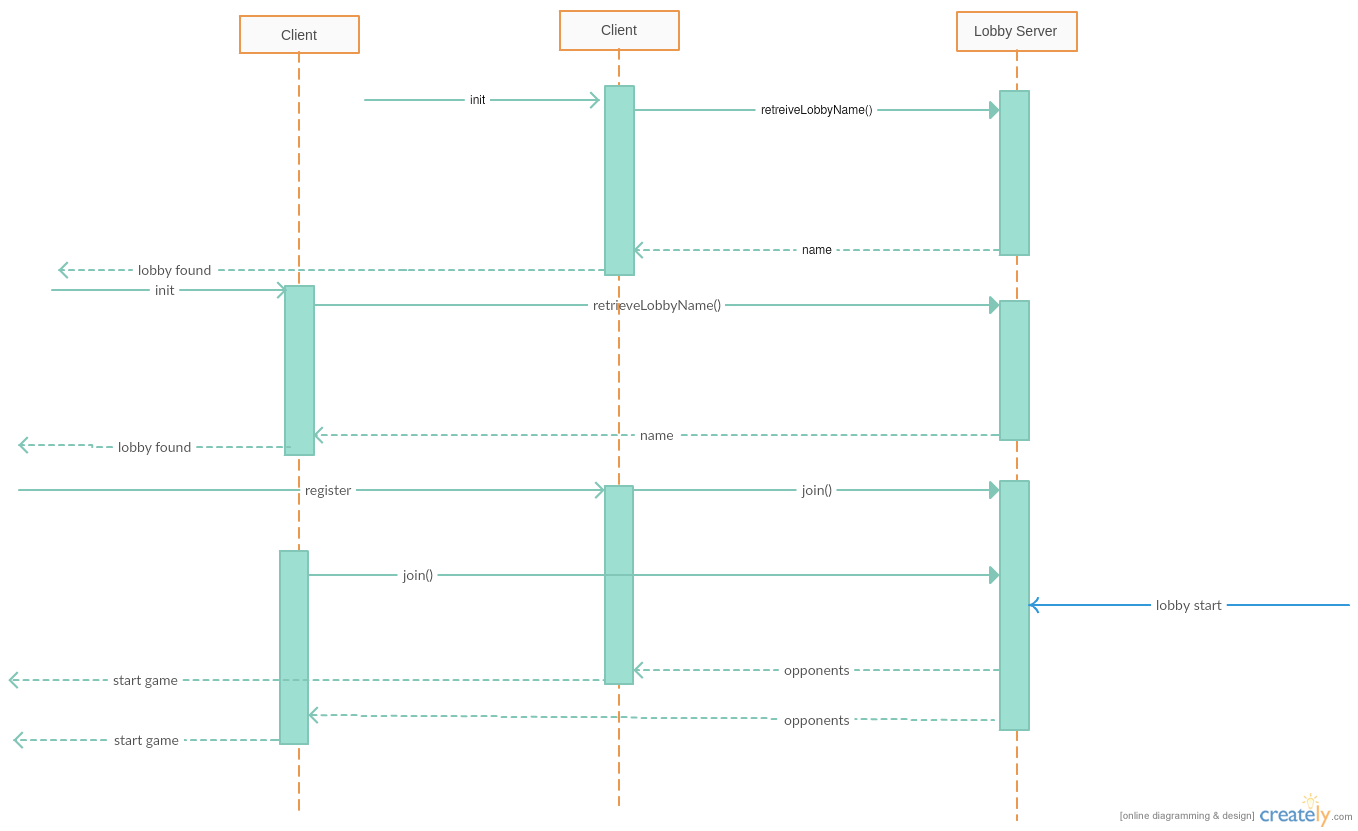
\includegraphics[width=0.8\textwidth]{core/imgs/UML/sequence/discovery.png}
    \caption{Diagramma delle interazioni, fase di discovery e registrazione}
    \label{fig:discoveryseq}
\end{figure}
Tramite il diagramma delle interazioni in figura \ref{fig:discoveryseq} 
è facile intuire come le fasi di discovery e registrazione siano legate 
indissolubilmente: durante la discovery il client trova una o più lobby, a cui 
poi richiede di unirsi. Come si evince dalla figura la discovery è una singola 
RMI, nella quale la lobby restituisce il suo nome (ed, implicitamente, il 
proprio IP). Durante la fase di join i vari client richiedono di unirsi alla 
lobby, successivamente è l'amministratore della lobby a dare il via alla 
partita da interfaccia grafica. Ai client viene quindi restituita la lista di 
giocatori (serializzati dall'oggetto NetPlayer) completa di indirizzi IP e 
porte. Si vedano in particolare i diagrammi delle classi in figure \ref{fig:classlobby}
e \ref{fig:classlobbyclientside} che descrivono l'implementazione della comunicazione con la lobby,
rispettivamente lato server e lato client.
\\
Per quanto riguarda l'implementazione della comunicazione fra client, essa è descritta dal
diagramma delle classi in figura \ref{fig:classgame}.
Prima di procedere con il gioco vero e proprio, tramite un'interfaccia 
TurnOrderinterface ciascun client si connette ai propri avversari e richiede ad 
essi un numero pseudocasuale, che viene usato per stabilire l'ordine di gioco 
nel modo seguente: il numero restituito viene concatenato al nome utente 
dell'avversario, l'ordine alfabetico di tali stringhe concatenate viene usato 
poi per ordinare la lista di giocatori. In questo modo si ha un tie-breaker nel 
caso in cui i numeri pseudo casuali siano uguali.
\\
\begin{figure}[!ht]
    \centering
    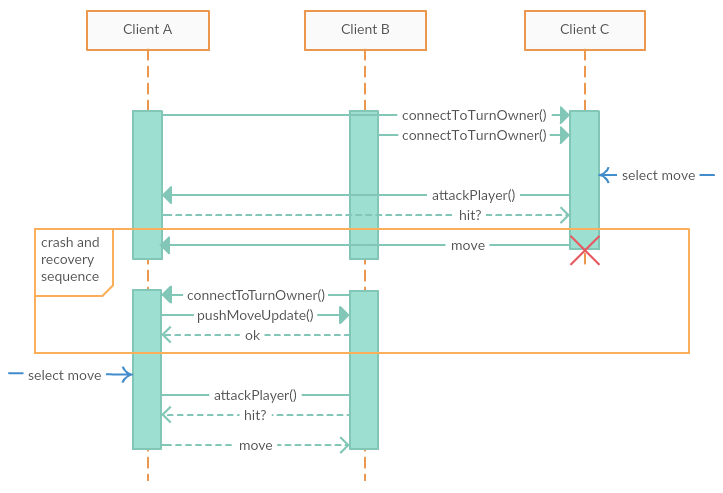
\includegraphics[width=0.8\textwidth]{core/imgs/UML/sequence/game.png}
    \caption{Diagramma delle interazioni, fase di gioco con crash e ritorno 
della mossa parziale}
    \label{fig:gameseq}
\end{figure}
Può dunque iniziare la fase di gioco vera e propria (fig \ref{fig:gameseq}): è 
la TurnOwnerInterface 
che fornisce ai client la possibilità di connettersi al giocatore il cui turno 
è appena iniziato per conoscerne la mossa. Esso effettua una prima 
sincronizzazione a barriera, per controllare il numero degli utenti connessi e 
conoscere l'ultima mossa che essi hanno ricevuto. Dopo tale sincronizzazione, 
il turn owner effettua una chiamata a metodo remoto implementata da una 
PushMoveInterface in modo da aggiornare, se necessario, i client che non hanno 
ricevuto l'ultima mossa (come avviene fra client A e B nella figura 
\ref{fig:gameseq}). Vi è dunque una seconda sincronizzazione a barriera, 
in attesa che tutti conoscano l'ultima mossa. L'utente sceglie dunque la 
mossa e l'avversario da attaccare, mentre a livello di comunicazione il turn 
owner contatta l'avversario selezionato (target) e richiede lo stato della 
cella selezionata nel suo campo di gioco. Il turno è dunque finito e il turn 
owner può restituire la mossa effettuata e il risultato di tale mossa agli 
altri giocatori, che sono ancora in attesa di risposta.
\\
Trattiamo ora brevemente le classi principali di errore che possono emergere a 
causa di crash dei client e le contromisure adottate per gestirle. Nel caso di 
un crash del turn owner, i client ad esso connessi sono notificati 
immediatamente da un'eccezione nella chiamata a metodo remoto. Il gioco può 
dunque proseguire tranquillamente dal prossimo giocatore in ordine, con le 
accortezze già descritte nel caso in cui non vi sia consistenza globale 
sull'ultima mossa effettuata. Il caso successivo è quello del crash di un altro 
client che non sia il turn owner. Tale crash non viene rilevato immediatamente 
se avviene dopo la prima sincronizzazione a barriera del turn owner. In questo 
caso è stato previsto che possa avvenire un attacco ad un client crashato, che 
causa un errore e la rimozione di quest'ultimo dalla lista dei giocatori del 
turn owner. Nel caso in cui il crash avvenga prima della sincronizzazione a 
barriera, il turnOwner attende un timeout di 500 %FIXME 
millisecondi e poi assume che i client che non si sono ancora connessi siano 
crashati. Si noti che il turn owner fornisce agli altri client una lista di 
player crashati, in modo che essi sappiano chi è ancora attivo alla fine di 
ciascun turno. Tramite tali accorgimenti il numero di player attivi è noto al 
turn owner all'inizio del proprio turno e viene comunicato a tutti alla fine di 
quest'ultimo. Vi possono essere dunque dei brevi periodi di tempo nei quali non 
è noto quali client siano ancora in esecuzione, tuttavia tali inconsistenze non 
creano problemi alla procedura di gioco e sono velocemente risolte all'inizio 
del turno successivo.
\\
È interessante evidenziare, infine, come vi sia una sostanziale equivalenza fra 
giocatori che hanno perso la partita e giocatori crashati: in entrambi i casi 
essi vengono estromessi dalla partita e semplicemente non ne fanno più parte.